% !TEX TS-program = xelatex
\documentclass{article}

\usepackage{amsmath}
\usepackage{esvect}
\usepackage{unicode-math}

\usepackage{listingsutf8}
\usepackage{color}

\definecolor{mygreen}{rgb}{0,0.6,0}
\definecolor{mygray}{rgb}{0.5,0.5,0.5}
\definecolor{mymauve}{rgb}{0.58,0,0.82}

\lstset{ %
  backgroundcolor=\color{white},   % choose the background color
  basicstyle=\footnotesize,        % size of fonts used for the code
  breaklines=true,                 % automatic line breaking only at whitespace
  captionpos=b,                    % sets the caption-position to bottom
  commentstyle=\color{mygreen},    % comment style
  escapeinside={\%*}{*)},          % if you want to add LaTeX within your code
  keywordstyle=\color{blue},       % keyword style
  stringstyle=\color{mymauve},     % string literal style
}

\usepackage{tkz-euclide}
\usetikzlibrary{calc, angles, quotes}

\usepackage{graphicx}
\graphicspath{{assets/}}

\usepackage{polyglossia}
\usepackage{hyperref}

\usepackage{multicol}

\usepackage{ragged2e}
\let\raggedright\RaggedRight

\hypersetup
{
  pdftitle   = {Computer Vision – Assignment 2},
  pdfauthor  = {Markus Reiter}
}

\title{Computer Vision – Assignment 2}
\author{Markus Reiter (in cooperation with Lukas Dötlinger)}

\begin{document}
\raggedright

  \maketitle

  \section{Rigid Transformation}

  \begin{multicols}{2}
    If we have a triangle $\Delta$ where

    \[
      \Delta =
      \begin{pmatrix}
        0 & 0 & 2 \\
        0 & 2 & 0 \\
        1 & 1 & 1
      \end{pmatrix}
    \]

    and translate it with translation matrix

      \[
        T =
        \begin{pmatrix}
          1 & 0 & 2 \\
          0 & 1 & 2 \\
          0 & 0 & 1
        \end{pmatrix}
      \]

    we get

    \[
      \Delta_T =
      \begin{pmatrix}
        2 & 2 & 4 \\
        2 & 4 & 2 \\
        1 & 1 & 1
      \end{pmatrix}
    \]

    \columnbreak

    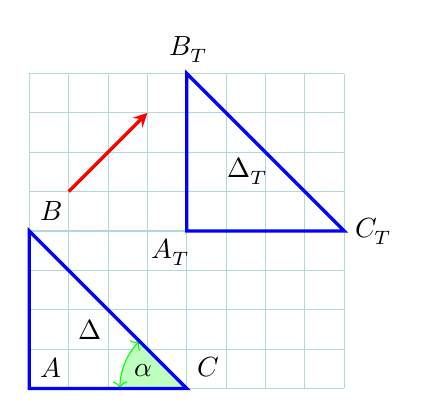
\begin{tikzpicture}
      \tkzInit[xmax = 4, ymax = 4, xmin = 0, ymin = 0]
      \tkzAxeXY

      \coordinate (A) at (0, 0);
      \coordinate (B) at (0, 2);
      \coordinate (C) at (2, 0);

      \draw[help lines] (0, 0) grid[step = 0.5] (4, 4);

      \pic [draw = green, text = black, fill = green!25, <->, "$\alpha$", angle eccentricity = 0.7, angle radius=0.85cm] {angle = B--C--A};


      \draw[very thick, blue, text = black] (A) node[above right] {$A$}
        -- (B) node[above right] {$B$}
        -- (C) node[above right] {$C$}
        -- cycle
      ;
      \tkzText[above right](0.5,0.5){$\Delta$}

      \draw[very thick, blue, text = black] ($ (A) + (2, 2) $) node[below left, xshift = 4pt, yshift = 1pt] {$A_T$}
        -- ($ (B) + (2, 2) $) node[above] {$B_T$}
        -- ($ (C) + (2, 2) $) node[right] {$C_T$}
        -- cycle
      ;
      \tkzText[above right, xshift = -3pt, yshift = -1pt](2.5, 2.5){$\Delta_T$}

      \draw[very thick, ->, >=stealth, red] (0.5, 2.5) -- (1.5, 3.5);
    \end{tikzpicture}
  \end{multicols}

  We then check if the distances stay the same.

  \begin{align*}
    \vv{AB} =&
    \begin{pmatrix}
      0 \\ 
      2
    \end{pmatrix}
    -
    \begin{pmatrix}
      0 \\ 
      0
    \end{pmatrix}
    \quad
    =
    \quad
    \begin{pmatrix}
      0 \\ 
      2
    \end{pmatrix}
    \quad
    =
    \quad
    \begin{pmatrix}
      2 \\ 
      4
    \end{pmatrix}
    -
    \begin{pmatrix}
      2 \\ 
      2
    \end{pmatrix}
    =
    \vv{A_TB_T}
    \\
    \vv{AC} =&
    \begin{pmatrix}
      2 \\ 
      0
    \end{pmatrix}
    -
    \begin{pmatrix}
      0 \\ 
      0
    \end{pmatrix}
    \quad
    =
    \quad
    \begin{pmatrix}
      2 \\ 
      0
    \end{pmatrix}
    \quad
    =
    \quad
    \begin{pmatrix}
      4 \\ 
      2
    \end{pmatrix}
    -
    \begin{pmatrix}
      2 \\ 
      2
    \end{pmatrix}
    =
    \vv{A_TC_T}
  \end{align*}

  We also check if the angles stay the same.

  \begin{align*}
    tan^{-1}\left(\frac{\lvert\vv{AB}\rvert}{\lvert\vv{AC}\rvert}\right)
    =
    tan^{-1}\left(\frac{2}{2}\right)
    \quad
    =
    \quad
    45°
    =
    \alpha
    \quad
    =
    \quad
    tan^{-1}\left(\frac{2}{2}\right)
    =
    tan^{-1}\left(\frac{\lvert\vv{A_TB_T}\rvert}{\lvert\vv{A_TC_T}\rvert}\right)
  \end{align*}

  This shows that translation preserves distances and angles.

  Since rotation is also a rigid transformation, the example above shows that rotation also preserves distances and angles, since all rigid tranformations have the same rules and properties.

  \section{RANSAC}

  \subsection*{a)}

  In the paper an algorithm called \textbf{RANSAC} is described, which stands for random sample consensus. It is an approach for solving the LDP (location determination problem). The paper starts out by explaining the problem and hence why we need this algorithm.

  What follows is a more detailed description of the algorithm and how it works. Then, the LDP itself is explained more in-depth and as well as how to go about solving it.

  The LDP with $n$ coordinates is called the PnP (perspective n-point problem). It is possible to have a non-unique solution for the PnP where $n \geq 3$.

  The next part shows the implementation of the \textbf{RANSAC/LD} algorithm.

  \subsection*{b)}

  \textbf{RANSAC} tries to solve the LDP, whose objective is to map points on an image to a set of landmarks with known locations.

  A reasonable computational load is guaranteed by using a small enough set of landmarks, but in order to avoid non-unique solutions, the set of landmarks has to be big enough. \textbf{RANSAC} als tries to solve the classification problem, where the objective is to find the best match between data and available objects. In addition, it also tries to solve the parameter estimation, that is choosing the best value for the parameters of the selected model. Gross errors cannot be detected or rejected by classical methods, this is what \textbf{RANSAC} overcomes. Smoothing techniques can handle small errors, but classification errors are critical and hence always seen as gross errors.

  \subsection*{c)}

  The first step for solving the LDP is to find the length of the three remaining legs of the tetrahedron ($\mathit{a, b, c}$) when the base ($\mathit{Rab, Rac, Rbc}$) and face angle of the opposite trihedral angle ($\theta{}ab,\ \theta{}ac,\ \theta{}bc$) are given. Using the law of cosine, this can be done by creating an equation system with the triangles between the camera position and two points of the consensus set, respectively.

  An equation in this system would look like

  \begin{align*}
    (Rab)^2 = a^2 + b^2 - 2 a b \cdot cos(\theta a b)
  \end{align*}

  Here, $Rab$ is the distance between points $A$ and $B$.

  P1P and P2P have infinite solutions, so in the paper, P6P is used to solve the LDP using an additional point inside of the triangle. Hence, a unique solution can be obtained with a consensus set of 6 landmarks.

  To detect and reject gross errors, \textbf{RANSAC} uses a random subset of points large enough and finds all points that meet the model within the given error radius. If a consensus set has been found, it is saved. This is repeated a number of times and at the end, the model with the smallest radius is chosen.

  \textbf{RANSAC/LD} is introduced in order to limit the number of gross errors. A threshold $t$ radius is determined from the input data. The probability $w$ for getting an error free data set is also given as input data. The maximum number of iterations $k$ needed for a given probability is

  \begin{align*}
    k = \frac{log(1 - t)}{log(1 - w^3)}
  \end{align*}

  \subsection*{d)}

  The algoritm is demonstrated with three experiments.

  \begin{enumerate}
    \item In a specific LDP was solved successfully with \textbf{RANSAC}, but couldn't be solved with the common least-squares heuristic.
    \item In order to check reliability, 50 synthetic problems with a wide variety of parameters values were solved using \textbf{RANSAC}.
    \item A real-world experiment in which landmarks were located by standard feature detection was conducted. These were then used to calculate the camera position and orientation using \textbf{RANSAC}.
  \end{enumerate}

  These examples give a good estimate of the capabilities of \textbf{RANSAC}.


  \newpage

  \section{Spatiotemporal Filtering}

  The purpose of this assignment was to extract motion from a video, that is, separating the static parts of a video from the ones containing motion. The hypothesis here is that we can detect motion by comparing the pixels of multiple frames of a video. If pixels with the same brightness stay at the same position, there is no motion, if they move to a different position, there is. To make this difference visible, we can interpolate over multiple frames. This is exactly the purpose of a spatiotemporal filter. It is applied on one axis, either x or y, and the time-axis which in case of videos consists of frames.

  Our solution was implemented in Matlab. We used \texttt{VideoReader} to read the video file as a matrix, after which we converted every frame to grayscale using \texttt{rgb2gray}. All frames were then concatenated to a \texttt{frames} vector.

  The second part was the function \texttt{energyOfGabor(video, gabor\_size, sigma, theta)}. In this function, a Gabor filter is generated using the function given in the assignment and using the variables passed to \texttt{energyOfGabor}. The \texttt{video} variable corresponds to the \texttt{frames} variable, which is ordered like this: \texttt{[height, width, frame]}. We then use \texttt{size(video, 2)} to get the width, in order to be able to loop through the x-axis. In each iteration of this loop, we then have a matrix of \texttt{[height, frame]} pixels, i.e. a column of the video. We get this column using \texttt{squeeze(video(:, col, :))}, and convolve it once using \texttt{g\_even}, and once using \texttt{g\_odd} with the \texttt{conv2} function. We then take the sum of the square of both of these, and then take the square root. We append the resulting column to an array. This array will have the form \texttt{[height, frame, width]}, so we have to permutate it once using the \texttt{permutate} function in order to look like the input array: \texttt{[height, width, frame]}.

  For the Nine-Tap filter, we use the same approach as for the \texttt{energyOfGabor} function. Inside the loop, we convolve one with our filter \texttt{f1}, and once with the filter \texttt{f2}. We then do an element-wise multiplication of the two resulting columns and append them to the output array.

  In our main program, either \texttt{energyOfGabor} or \texttt{nineTap} is called and its result is displayed with \texttt{implay}.

  \subsection{Results}

  With the Gabor filter, there is a clear distinction between moving and still parts of a video. In our case, we used a Gabor filter of size 9, which gave the best result. The Nine-Tap filter does have a lot of noise, which is presumably because it is only a filter of size 3, but even though there is a lot of noise, the motion can be clearly distinguished from the noise.

  \begin{figure}[!ht]
    \caption{Energy of Gabor}
    \centering
    \includegraphics[width=.8\textwidth]{gabor.png}
  \end{figure}

  \begin{figure}[!ht]
    \caption{Nine-Tap Filter}
    \centering
    \includegraphics[width=.8\textwidth]{nine-tap.png}
  \end{figure}

  \clearpage

  \appendix

  \section*{Appendix A}

  \begin{figure}[!ht]
    \lstinputlisting[language = matlab, caption = task3.m]{task3.m}
  \end{figure}


  \begin{figure}[!ht]
    \lstinputlisting[language = matlab, caption = gaborEnergy.m]{gaborEnergy.m}
  \end{figure}

  \begin{figure}[!ht]
    \lstinputlisting[language = matlab, caption = gaborFilter.m]{gaborFilter.m}
  \end{figure}

  \begin{figure}[!ht]
    \lstinputlisting[language = matlab, caption = nineTap.m]{nineTap.m}
  \end{figure}
\end{document}
